\chapter{Conclusions}\label{ch:conclusions}
In this work, progress was made on the creation of a mixed reality application dedicated to
teaching music in schools, especially in the first approach to the subject.
The work starts with an existing prototype, which had the shortcoming of requiring a computer and specific hardware
to run, and brings it to a mobile device, a smartphone, accessible to all and available at affordable prices.
The software can also run without problems on cheap and not too recent devices,
while still achieving performance similar to that of top-of-the-range devices.

The biggest improvements were found in the general usability of the application, thanks to the porting to smartphones
and the elimination of all external hardware, and in the keyboard detection algorithm,
which achieves almost perfect results on any type of keyboard without the need for any special lighting measures
and now consists of a single step.

Some progress was made also in the playing phase, which is now more precise and reliable on average,
but there is still much room for improvement.


\section{Future development}\label{sec:future-development}
In the next stages of development we plan to improve the touch recognition algorithm
to achieve better precision and accuracy.
This will be done by completely changing the keyboard detection phase from the current single-shot phase to a slightly
longer procedure, but one that we hope will lead to better results.

The idea is to use plane detection techniques to locate the table with the paper on it, do the keyboard detection
from above, and then move the phone to a very low angle, almost parallel to the table, tracking the position of the
paper (and thus the keyboard) in 3D space while the phone moves to the new position.

This would allow us to have a perfect view of the distance of the fingers from the sheet, greatly increasing the
accuracy of touch recognition, while maintaining full information on the position of the keys thanks to plane
detection and tracking of the sheet during the transition from 90\degree \ to the flat position.

Plane detection and keyboard tracking can be made very accurate by the fact that the size of the sheet is known,
being an ordinary A4 sheet.
View from the flat position is shown in~\autoref{fig:future-work}.

As an alternative to the above strategy, it would be possible to develop an ad-hoc neural network,
suitable for running on mobile devices, with the aim of detecting, from the RGB image alone,
which fingers are pressed on the surface of the sheet.
This neural network, if developed, will be trained with a dataset of images of hands in different positions and with
different fingers pressed, and will be able to return, for each frame, which fingers are pressed and on which keys.

We also plan to assess the feasibility of porting it to iOS, to expand the pool of users that our application can reach.

\begin{figure}[ht]
	\centering
	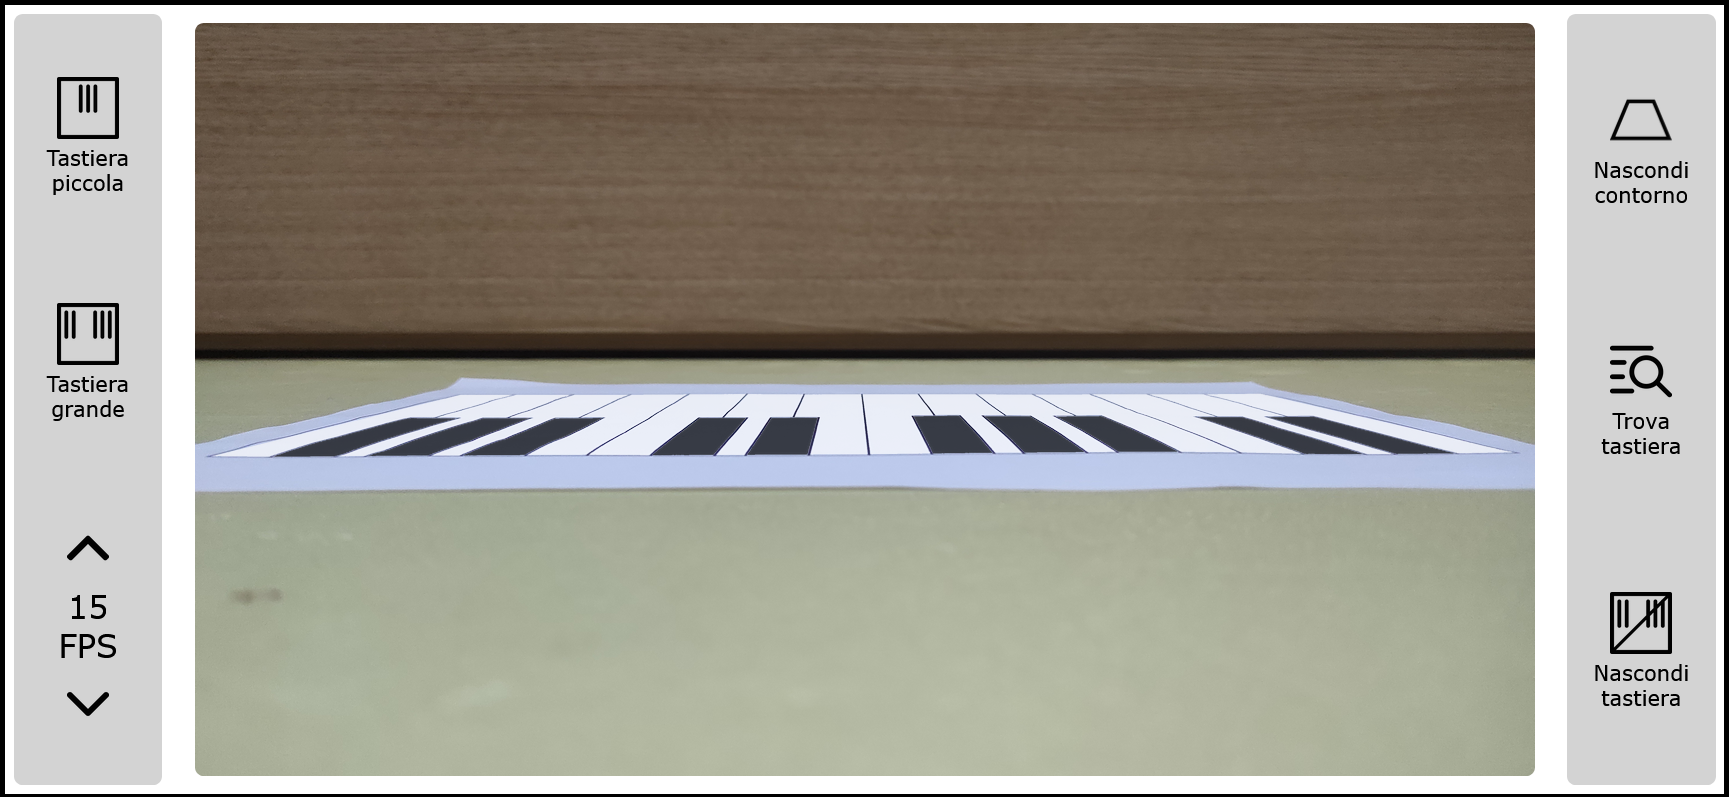
\includegraphics[width=\textwidth]{images/application/screenshots/playing-phase-flat}
	\caption{Flat view of the keyboard, still in development.}
	\label{fig:future-work}
\end{figure}
